\chapter{前庭系统} \label{chap:chap27}

现代交通工具在地球上的旅行和穿越地外空间的旅行依赖复杂的制导系统,该系统通过传感器、计算算法和卫星三角测量整合加速度、速度和位置信息。
然而,惯性制导的原理是古老的:脊椎动物使用类似系统已有 5 亿年历史,无脊椎动物使用时间更长。
在这些动物中,惯性制导系统(称为前庭系统\footnote{名称来源于其在内耳中的位置,描述内耳中位于耳蜗和半规管之间的空腔结构(前厅)。})用于检测和解释空间运动以及相对于重力的方向。


通过数十年的广泛研究,很明显地球上的大多数(如果不是全部)生物体已经进化到能够感知我们宇宙中最普遍的“力”之一,即引力。
感觉转导的机制与大自然所能设计的一样多样。
重力最准确的名称是\textit{重力-惯性加速度},这是一种指向我们地球核心的独特形式线性加速度。
事实上,重力在赤道和两极之间系统地变化多达 0.5\%;
在地球表面矿物质密集的地区重力会增加,而在矿物质较少的地区重力会减少。
然而,动物执行的每一个行为都参考了\textit{重力-惯性加速度},我们所有的行为和认知指令都取决于我们的运动和相对于它方向的知识。
我们所说的前庭系统第一个发育实际上是重力传感器。
随着行为变得越来越灵活,感觉器官也进化为处理旋转加速度。


在本章中,我们将集中讨论脊椎动物的前庭系统,该系统在许多物种中都保持高度保守。
如图~\ref{fig:27_1}B~所示,前庭信号起源于内耳的迷路。
骨迷路是颞骨岩部内的中空结构。
它内部是膜状迷路,其中包含前庭系统和听觉系统的传感器。


\begin{figure}[htbp]
	\centering
	\includegraphics[width=0.84\linewidth]{chap27/fig_27_1}
	\caption{内耳的前庭器官。
		A. 内耳的前庭和耳蜗部分的方向相对于头部显示。
		B. 内耳分为骨迷路和膜迷路。
		骨迷路以颞骨的岩骨部分为界。
		位于该结构内的是膜迷路,其中包含听觉器官(耳蜗)和平衡器官(椭圆囊、球囊和半规管)。
		骨和膜之间的空间充满外淋巴,而膜迷路充满内淋巴。
		半规管的椭圆囊、球囊和壶腹中的感觉细胞对头部的运动作出响应\cite{iurato2013submicroscopic}。}
	\label{fig:27_1}
\end{figure}


前庭受体由 2 部分组成:2 个耳石器官,椭圆囊和球囊(测量线性加速度),以及 3 个半规管(测量角加速度)。
旋转运动(角加速度)发生在头部转动、身体旋转以及主动或被动运动期间,而线性加速度发生在行走、跌倒、车辆行驶(即平移)或相对于重力的头部倾斜过程中。
这些受体将前庭系统的信息发送到大脑,在那里它被整合成关于运动方向和速度以及头部相对于\textit{重力-惯性加速度}位置的适当信号。
在与受体传入纤维的第一个连接处的许多中枢前庭神经元也接收来自其他系统的汇聚信号,例如\textit{本体感受器}、视觉信号和运动命令。
这些多模态信号的中央处理发生得非常快,以确保视觉凝视和姿势响应、自主响应和空间方向意识的充分协调。



\section{内耳的前庭迷路包含 5 个受体器官}

膜迷路由结缔组织的丝状网络支撑在骨迷路内。
膜迷路的前庭部分位于耳蜗的外侧和后方。
如图~\ref{fig:27_1}B~所示,前庭受体包含在膜迷路的专门扩大区域中,称为半规管的壶腹和耳石器官的斑块。
2 个耳石器官都位于膜迷路的中央隔间(前庭),它被同名的骨迷路包围。


膜迷路充满了内淋巴(一种 150 毫摩尔的富含~\ce{K+}和16 毫摩尔的缺乏~\ce{Na+}液体),其成分由专门细胞中离子泵的作用维持。
内淋巴沐浴在前庭受体细胞的表面。
在膜迷路周围,在膜迷路和骨迷路壁之间的空间中,是外淋巴。
外淋巴是一种高~\ce{Na+}(150 毫摩尔)、低~\ce{K+}(7 毫摩尔)的液体,其成分与脑脊液相似,并通过耳蜗管与脑脊液相通。
外淋巴浸润受体上皮细胞和前庭神经纤维的基底表面。
如图~\ref{fig:27_1}B~所示,骨迷路中的 2 个液密分区(椭圆形和圆形窗口)将外淋巴空间连接到中耳腔。
卵圆窗通过中耳听小骨与鼓膜相连。
这些窗口对于声音传导很重要(第~\ref{chap:chap26}~章)。
内淋巴和外淋巴通过围绕每个受体细胞顶端的支持细胞的连接复合体保持分离。
由于外伤或疾病破坏这 2 种液体之间的平衡会导致前庭功能障碍,导致头晕、眩晕和空间定向障碍。


在发育过程中,迷路从一个简单的囊发育为一组复杂的相互连接的感觉器官,但保留了相同的基本拓扑结构。
每个器官都起源于从耳囊中萌发的上皮内衬囊袋,并且几个器官内的内淋巴空间在成人中保持连续。
如图~\ref{fig:27_1}B~所示,前庭迷路的内淋巴空间也通过\textit{连合管}连接到耳蜗管。
此外,膜迷路包含一个小管(即内淋巴管),它延伸穿过S型骨中的一个空间(即前庭导水管)终止于后颅窝硬膜外间隙中与硬脑膜相邻的盲囊。
人们认为内淋巴囊具有吸收和排泄功能以维持内淋巴液的离子组成。


\subsection{毛细胞将加速刺激转化为受体电位}

5 个受体器官中的每一个都有一组毛细胞,负责将头部运动转换为前庭信号。
毛细胞因排列着近 100 个交错高度的静纤毛而得名。
最短的静纤毛在细胞的一端,最高的在另一端,以毛细胞唯一真正的纤毛结束,称为动纤毛。
动纤毛通常是所有静纤毛中最高的。
如图~\ref{fig:27_2}~所示,头部的角加速度或线加速度导致静纤毛偏转,静纤毛共同组成了\textit{发状纤维束}。


\textit{发状纤维束}静纤毛尖端的专门离子通道允许~\ce{K+}进入或被周围的内淋巴阻断(第~\ref{chap:chap26}~章)。
如图~\ref{fig:27_2}~所示,这个动作允许毛细胞充当机械受体,其中静纤毛的偏转产生去极化或超极化受体电位,具体取决于\textit{发状纤维束}移动的方向。
如图~\ref{fig:27_2}~所示,受体膜的这些去极化和超极化分别导致神经支配传入神经的激发率和抑制率。
在每个前庭受体器官中,毛细胞的排列使得运动方向特异性由某些细胞的兴奋和其他细胞的抑制来定义。

\begin{figure}[htbp]
	\centering
	\includegraphics[width=0.8\linewidth]{chap27/fig_27_2}
	\caption{前庭迷路中的毛细胞将机械刺激转化为神经信号。
		在每个细胞的顶端是静纤毛,其长度向单个动纤毛方向增加。
		受体细胞的膜电位取决于静纤毛弯曲的方向。
		向动纤毛偏转导致细胞去极化,从而增加传入纤维的放电率。
		远离动纤毛弯曲导致细胞超极化,从而降低传入放电率\cite{flock1965transducing}。}
	\label{fig:27_2}
\end{figure}


前庭蜗神经(第 8 对颅神经)的分支将前庭信号从毛细胞传送到脑干,前庭蜗神经进入脑干并终止于同侧前庭核、小脑和网状结构。
如图~\ref{fig:27_1}A~所示,前庭神经的细胞体位于内耳道内的\textit{斯卡帕神经节}。
前庭上神经支配水平和前管以及囊,而前庭下神经支配后管和球囊。
迷路的血管供应起源于小脑前下动脉,随第 8 神经行进。
前庭前动脉供应前庭上神经支配的结构,前庭后动脉供应前庭下神经支配的结构。


所有脊椎动物受体毛细胞都接收来自脑干的传出输入。
前庭受体的传出神经支配的功能仍然是一个争论的话题。
刺激来自脑干的传出纤维会改变来自毛细胞的传入轴突的敏感性。
它增加了一些传入神经和毛细胞的兴奋性,同时抑制了其他传入神经和毛细胞,并且因物种而异。



\subsection{半规管感知头部旋转}

当物体绕轴的旋转速率发生变化时,物体会经历角加速度。
因此,头部在旋转或倾斜时、身体旋转时以及主动运动或被动移动期间都会经历角加速度。
每个前庭迷路的 3 个半规管检测这些角加速度,并向大脑报告它们的大小和运动方向。


每个半规管都是从前庭延伸的半圆形膜迷路管。
每根管的一端通向前庭,而在另一端(即壶腹),管的整个内腔被液密的凝胶状隔膜(即壶腹横穿)。
如图~\ref{fig:27_3}~所示,静纤毛和动纤毛伸入凝胶状杯状部,而毛细胞位于受体上皮细胞嵴下方,连同支配神经的传入神经末梢。


\begin{figure}[htbp]
	\centering
	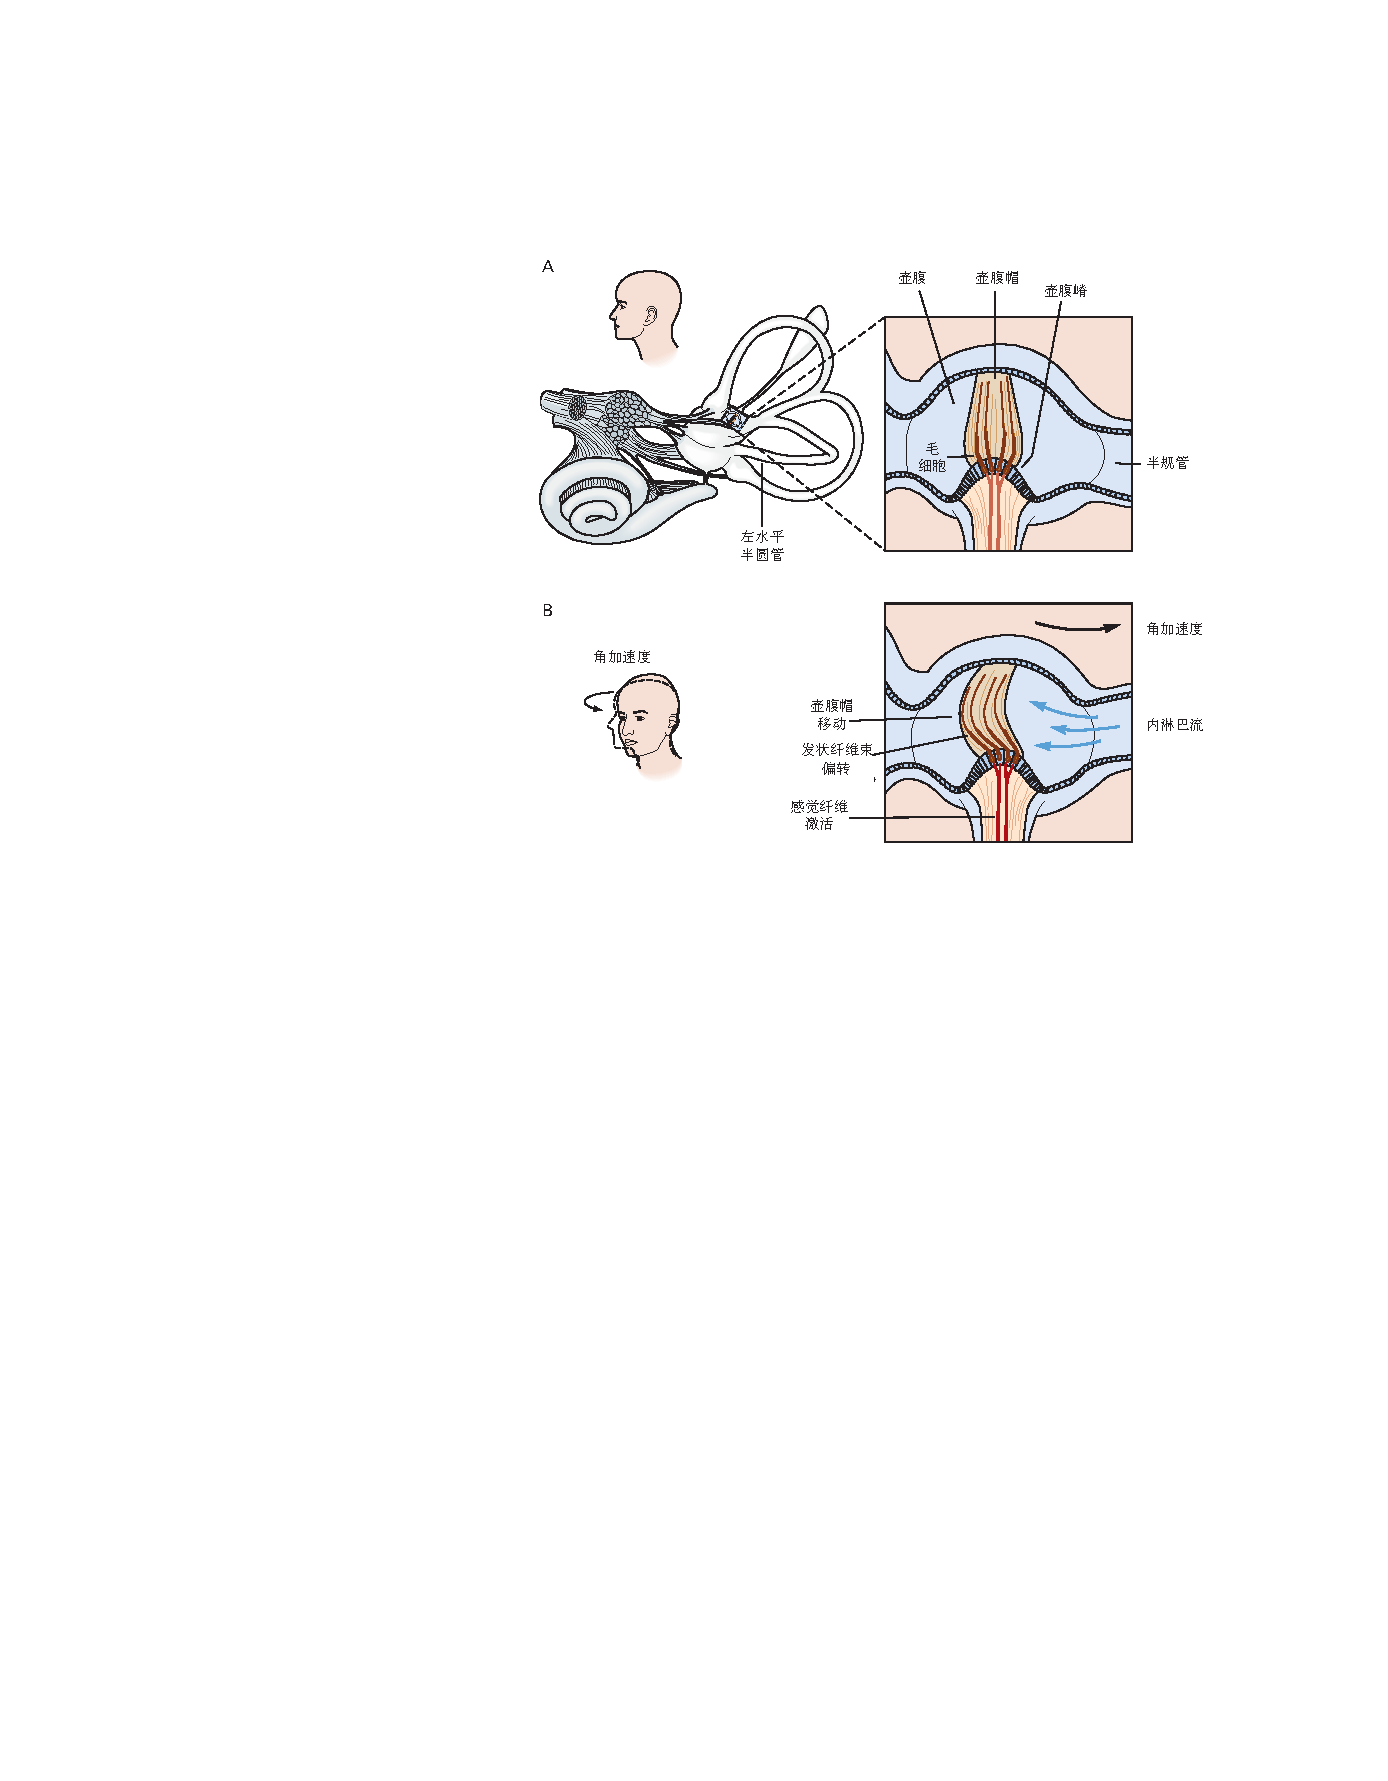
\includegraphics[width=0.89\linewidth]{chap27/fig_27_3}
	\caption{半规管的壶腹。
		A. 上皮增厚区(即壶腹嵴)包含毛细胞。
		毛细胞的静纤毛和动纤毛延伸到凝胶状的隔膜(即壶腹),该隔膜从\textit{壶腹嵴}延伸到壶腹顶部。
		B. 当头部转动时,内淋巴的相对运动会使\textit{壶腹帽}移位。
		结果,\textit{发状纤维束}也移位了。
		图中大大夸张了他们的运动。}
	\label{fig:27_3}
\end{figure}


前庭器官检测到头部的加速度,因为内淋巴和吸盘的惯性导致作用在静纤毛上的力。
考虑最简单的情况,即半规管平面内的旋转。
当头部开始旋转时,膜迷路和骨迷路随之移动。
然而,如图~\ref{fig:27_3}B~所示,因为内淋巴的惯性,它滞后于周围的膜迷路,从而将壶腹推向与头部相反的方向。


半规管中内淋巴的运动可以用一杯咖啡来证明。
在围绕其垂直轴轻轻转动杯子的同时,观察流体外边界附近的特定气泡。
当杯子开始转动时,咖啡往往会保持其在空间中的初始方向,从而在杯子中反向旋转。
如果你继续以相同的速度旋转杯子,咖啡(和气泡)最终会追上杯子并随之旋转。
当杯子减速并停止时,咖啡继续旋转,相对于杯子向相反的方向移动。


在壶腹中,内淋巴的这种相对运动会在壶腹上产生压力,使其弯曲朝向或远离相邻的前庭,这取决于内淋巴流动的方向。
由此产生的静纤毛偏转会改变毛细胞的膜电位,从而改变相关感觉纤维的放电率。
每个半规管对其平面内的旋转最为敏感。
水平管位于鼻枕轴上方约 30°(当人行走并注视前方地面时大致处于水平面),因此对水平面的旋转最为敏感。
静纤毛的排列使得向左的旋转运动对左侧水平管是兴奋的,对右侧水平管是抑制性的。
如图~\ref{fig:27_4}~所示,前后管在头部更垂直,与矢状面成大约 45 度角。 
类似的在前管平面向下的旋转运动对前管毛细胞是兴奋的,而向上的头部运动是对后管的兴奋。


\begin{figure}[htbp]
	\centering
	\includegraphics[width=1.0\linewidth]{chap27/fig_27_4}
	\caption{双侧半规管对称。
		两侧的水平管道大致位于同一平面内,因此是功能对。
		双侧垂直管的关系更为复杂。
		一侧的前管和另一侧的后管位于平行平面内,因此构成功能对。
		垂直半规管与正中矢状面成近 45°。
		头部一侧的每个半规管位于彼此大致正交的平面内。}
	\label{fig:27_4}
\end{figure}


因为左右迷路近似镜像对称,所以 6 条管道有效地作为 3 个共面对运行。
2 条水平管道形成 1 对;
其他每对由头部一侧的一个前管和对侧的后管组成。
此外,如图~\ref{fig:27_4}~所示,头部两侧的 3 个半规管彼此大致正交。
当头部向受体毛细胞移动时(例如,头部向左转向左侧水平半规管),静纤毛向高动纤毛弯曲,从而刺激(去极化)细胞。
相反方向的头部运动导致远离运动纤毛并朝向最小的静纤毛弯曲,从而关闭通道并抑制(超极化)细胞。


左右耳半规管极性相反;
因此,当你向左转头时,左侧水平半规管中的受体会被兴奋(放电率增加),而右侧水平半规管中的受体会受到抑制(如图~\ref{fig:27_5}~所示,放电率降低)。
同样的关系也适用于垂直半规管。
管道平面也大致与特定眼部肌肉的牵拉平面对齐。
这对水平管道位于外侧和内侧直肌的牵拉平面上。
左前管和右后管对位于左上、下直肌和右上、下斜肌的牵引平面内。
右前和左后对占据左上、下斜肌和右上、下直肌的牵引平面。


\begin{figure}[htbp]
	\centering
	\includegraphics[width=0.8\linewidth]{chap27/fig_27_5}
	\caption{左右水平半规管共同作用以发出头部运动信号。
		由于惯性,逆时针方向旋转头部会导致内淋巴相对于管道顺时针移动。
		这使左侧管中的静纤毛偏向兴奋方向,从而刺激这一侧的传入纤维。
		在右管中,传入纤维超极化,因此激活减少。}
	\label{fig:27_5}
\end{figure}



\subsection{耳石器官感知线性加速度}

前庭系统不仅要补偿头部旋转,还要补偿线性运动。
椭圆囊和球囊这 2 个耳石器官检测线性运动以及头部相对于重力的静态方向,重力本身就是一个线性加速度。
每个器官由最长约 3 毫米的膜状迷路囊组成。
每个器官的毛细胞排列成一个大致呈椭圆形的斑块,称为黄斑。
人类椭圆囊包含大约 3 万个毛细胞,而球囊包含大约 1 万 6 千个。


如图~\ref{fig:27_6}~所示,耳石毛细胞的\textit{发状纤维束}延伸成凝胶状薄片,即覆盖整个黄斑的耳石膜。
嵌在该膜表面的是细密的碳酸钙颗粒,称为耳石。
耳石通常长 0.5 至 30 微米;
数以千计的这些颗粒附着在椭圆囊和球囊的耳石膜上。


\begin{figure}[htbp]
	\centering
	\includegraphics[width=1.0\linewidth]{chap27/fig_27_6}
	\caption{椭圆囊检测头部的倾斜。
		椭圆囊上皮中的毛细胞具有突出到耳石膜中的顶端\textit{发状纤维束},耳石膜是一种被数百万碳酸钙颗粒(耳石)覆盖的凝胶状物质。
		\textit{发状纤维束}是极化的,但朝向不同的方向。
		如图~\ref{fig:27_7}~所示,每个毛细胞的方向极性是相对于穿过椭圆囊中心的反转区域组织的,称为纹状体。
		因此,当头部倾斜时,作用在耳石上的重力会使每个\textit{发状纤维束}向特定方向弯曲。
		当头部向毛细胞极性轴的方向倾斜时,该细胞去极化并激活传入纤维。
		当头部向相反方向倾斜时,同一细胞超极化并抑制传入纤维\cite{iurato2013submicroscopic}。}
	\label{fig:27_6}
\end{figure}


\begin{figure}[htbp]
	\centering
	\includegraphics[width=0.67\linewidth]{chap27/fig_27_7}
	\caption{椭圆囊中每个毛细胞的机械敏感性轴都朝向纹状体。
		纹状体在包含毛细胞的黄斑表面弯曲,导致毛细胞群中机械敏感性轴(箭头)发生特征性变化。
		由于这种排列,向任何方向倾斜都会使一些细胞去极化并使其他细胞超极化,而对其余细胞没有影响\cite{spoendlin2016ultrastructure}。}
	\label{fig:27_7}
\end{figure}


重力和其他线性加速度对耳石基质和凝胶状耳石膜施加剪切力,它们可以相对于膜迷路移动。
这导致\textit{发状纤维束}偏转,改变前庭神经的活动,以发出由于平移运动或重力引起的线性加速度信号。
耳石器官的方向和单个毛细胞的方向敏感性使得可以感知沿任何轴的线性加速度。
例如,当头部处于正常位置时,每个椭圆囊的黄斑在鼻枕轴上方升高约 30°,类似于水平半规管。
在正常的头部休息位置,椭圆囊发生偏移,使椭圆囊与地球水平面大致相等。
如图~\ref{fig:27_6}~和图~\ref{fig:27_7}~所示,水平面上的任何加速度都会根据它们的方向激发每个椭圆囊中的一些毛细胞并抑制其他毛细胞。


成对球囊的运作类似于椭圆囊。
毛细胞代表每个囊状黄斑平面内所有可能的方向,但黄斑在近旁矢状平面中垂直取向。
因此,球囊对垂直加速度特别敏感。
某些囊状毛细胞也对水平面的加速度有响应,尤其是沿前后轴的加速度。



\section{前庭中央核整合前庭、视觉、本体感受和运动信号}

前庭神经从前庭神经节向同侧投射,主要到达位于第四脑室底部的脑桥和延髓背侧的 4 个前庭核(内侧、外侧、上部和降部)。
如图~\ref{fig:27_8}A~所示,许多前庭神经纤维也分叉,直接投射到顶核、结节和悬雍垂以及网状结构。
这些核将来自前庭器官的信号与来自脊髓、小脑和视觉系统的信号整合在一起。


\begin{figure}[htbp]
	\centering
	\includegraphics[width=1.0\linewidth]{chap27/fig_27_8}
	\caption{前庭核的传入纤维和中央投射。
		A. 来自前庭受体的传入纤维终止于脑干和小脑。
		来自半规管的纤维主要投射到前庭上核和内侧前庭核的内侧部分、\textit{前庭神经下核}、小脑(结节和悬雍垂)和网状结构。
		来自耳石的纤维主要投射到所有前庭核、结节和悬雍垂以及网状结构的外侧部分\cite{gacek1974localization}。
		B. 中央投射至前庭核来自许多大脑皮层、脑干和脊髓区域。
		这些包括前运动和多感觉皮层、辅助视神经核、小脑、神经整合核、网状结构、脊髓和来自对侧前庭核的连合纤维。}
	\label{fig:27_8}
\end{figure}


如图~\ref{fig:27_9}~所示,前庭核又投射到许多中央目标,包括动眼神经核、与凝视和姿势运动有关的网状和脊柱中枢,以及丘脑。
如图~\ref{fig:27_8}~和图~\ref{fig:27_9}~所示,许多前庭核神经元与小脑有相互联系,主要在絮状结节叶中,形成眼球运动、头部运动和姿势的重要调节机制。
如图~\ref{fig:27_8}~所示,前庭核接收来自\textit{前运动皮层}、辅助视神经系统(视束核)、神经整合核(舌前核和\textit{间位核})和网状结构的输入。
来自前庭核的进一步投射到达头侧和尾侧\textit{延髓}核,它们参与调节血压、心率、呼吸和\textit{骨重建},以及臂旁核以调节稳态。
最后,如图~\ref{fig:27_9}~所示,还有从前庭核到内侧膝状体(听觉)核的投射,以及膝上核和背侧被盖核,它们有助于空间定向。


\begin{figure}[htbp]
	\centering
	\includegraphics[width=0.65\linewidth]{chap27/fig_27_9}
	\caption{(左)前庭神经核的输出投射。
		前庭核投射到大脑皮层水平以下的许多大脑区域。
		两条独立的下行通路穿过\textit{外前庭脊髓束}和\textit{内侧前庭脊髓束},终止于脊髓。
		前庭核也投射到脑干中的网状结构和外侧延髓核。
		上行投射到膝上核、背侧被盖核、动眼神经核(外展神经、动眼神经和滑车神经)和神经积分器核(红线表示兴奋;灰线表示抑制),以及小脑的投射也是如此 (细胞核、结节和悬雍垂)。
		其他突出的前庭投射终止于膝状核和丘脑(腹外侧、后部和椎板内丘脑区域)。}
	\label{fig:27_9}
\end{figure}


如图~\ref{fig:27_8}~所示,前庭上核和内侧前庭核主要接收来自内侧区域半规管的纤维和外侧区域的一些耳石输入。
如图~\ref{fig:27_9}~所示,它们主要将纤维输送到小脑、网状结构、丘脑、动眼神经中枢和脊髓。
动眼神经中心输出包括 3 个动眼神经核(外展神经、动眼神经、滑车神经),以及用于将头部速度转换为舌下核(水平眼球运动)和\textit{间位核}(垂直眼球运动)中的头部位置信号的神经积分器。
稍后将更详细地描述这些核。


如图~\ref{fig:27_9}~和第~\ref{chap:chap35}~章所示,另一个与凝视控制有关的主要输出通路来自内侧前庭核(以及来自\textit{前庭神经下核}和外侧前庭核的较小投射),并通过内侧前庭脊髓束双侧投射到颈脊髓。
有两类内侧前庭脊髓纤维。
前庭脊髓神经元仅投射到脊髓以控制颈部肌肉组织。
前庭眼神经元投射到脊髓和动眼神经核,并参与协调眼球和头部运动以保持凝视稳定性。


外侧前庭核(\textit{戴特氏核})接收来自内侧半规管和外侧耳石器官的纤维。
如图~\ref{fig:27_9}~所示,通过外侧前庭脊髓束向同侧脊髓的所有水平提供主要输出,主要与通过调节肢体和轴向肌肉组织的姿势反射有关。
外侧前庭核神经元也大量投射到网状结构。
\textit{前庭神经下核}主要接收耳石输入,但也在内侧接收半规管纤维,并投射到小脑、网状结构和脊髓(内侧前庭脊髓束)。
兴奋性前庭核投射的主要神经递质包括谷氨酸,而抑制性投射是甘氨酸或\textit{$\gamma$-氨基丁酸}。
脊柱系统的前庭投射在第~\ref{chap:chap36}~章中有更详细的讨论。



\subsection{前庭连合系统传递双边信息}

如图~\ref{fig:27_8}B~所示,许多这些前庭核神经元通过使用\textit{$\gamma$-氨基丁酸}作为神经递质的抑制性连合通路接收来自对侧耳朵的会聚运动信息。
连合通路根据接收信息的受体类型高度组织。
例如,从同侧水平兴奋通道接收信号的细胞也将通过抑制性中间神经元从对侧水平通道接收信号。
由于每只耳朵中受体的方向选择性,在同侧头部转动过程中,对侧水平耳道输入总是会减少,实际上“解除抑制”来自对侧的抑制性输入。


连合系统的作用是增加前庭核神经元的响应并减少传入信号的噪音,从而产生“推拉”前庭功能。
从工程学的角度来看,核神经元中的“推拉”设定点不断更新来自对侧耳朵的耳道信号以充当比较器连接点,并可以解释耳道传入神经元的相对较高的自发放电率,接近 100 个脉冲/秒。
例如,在向左转头时,左脑干核神经元从左侧水平管接收高放电率信号,从右侧水平管接收低放电率信号。
如图~\ref{fig:27_5}~所示,活动的比较被解释为左转头。
对于来自一侧前半规管和另一侧耳侧后半规管的输入信号,也会出现类似的信号比较。
因此,对于任何头部平面中的旋转运动,比较器能够非常明确地确定运动方向。


左右耳道输入之间正常平衡的任何破坏(例如,来自受体器官或神经的外伤或疾病)将被大脑解释为头部旋转,即使头部是静止的。
这些影响通常会导致旋转或旋转的错觉,这些错觉可能会非常令人不安,并可能导致恶心或呕吐。
然而,随着时间的推移,连合纤维提供前庭补偿,单侧前庭受体功能的丧失在中枢部分恢复并且\textit{前庭-眼动反射}等行为响应大部分恢复的过程。



\subsection{联合半规管和耳石信号改善惯性感知并减少平移与倾斜的歧义}

在某些情况下,来自单个受体的前庭输入可能是模糊的。
例如,爱因斯坦\cite{einstein1908relativitatsprinzip}表明,无论线性加速度是由平移运动还是头部相对于重力的倾斜引起的,它们都是等价的。
如图~\ref{fig:27_10}~所示,耳石受体不能区分这两者:那么我们如何区分向右平移和向左倾斜,其中耳石传入信号的线性加速度是相同的。


\begin{figure}[htbp]
	\centering
	\includegraphics[width=0.56\linewidth]{chap27/fig_27_10}
	\caption{前庭输入信号的身体姿势和运动可能是模棱两可的。
		姿势系统无法仅根据耳石输入来区分身体的倾斜和线性加速度。
		作用在前庭毛细胞上的相同剪切力可由头部倾斜(左)产生,这使毛细胞暴露于\textit{重力}引起的\textit{加速度}的一部分,或来自身体的水平线性加速度(右边)。}
	\label{fig:27_10}
\end{figure}


现在已经确定,汇聚前庭核和小脑神经元使用来自半规管和耳石受体的组合信号以及一些简单的计算来区分倾斜和平移。
因此,一些中央前庭和小脑细胞编码头部倾斜,而其他细胞编码平移运动,正如我们将看到的,这对于控制头部和眼球运动极为重要。



\subsection{前庭信号是头部运动控制至关重要的组成部分}

一个重要的发现是一些前庭核神经元对主动产生和被动产生的头部运动的不同响应。
具体而言,与前庭传入相反,前庭核团和小脑中的一些神经元众所周知在被动运动期间对前庭刺激做出响应,但在自生运动期间会失去或降低其敏感性。
对被动运动或主动、和被动运动组合的被动成分的优先响应被解释为感觉预测误差信号:
大脑预测自生运动如何激活前庭器官并从传入信号中减去这些预测。
这种误差信号对于头部运动的在线控制以及头部运动估计很重要。


在计算上,这些属性已经使用所有感觉运动系统共有的概念进行了定量解释;
也就是说,主动运动信号和被动运动信号由运动传感器的内部模型(即耳道、耳石器官和颈部\textit{本体感受器})处理。
大脑使用物理定律和感觉动力学的内部表示(可以优雅地建模为传感器的前向内部模型)来处理前庭信号。
没有这样的误差信号,准确的自运动估计将受到严重损害。
这些计算见解表明,与早期解释不同,前庭信号在主动生成的头部运动期间与自我运动估计和头部运动控制相结合时仍然非常重要。



\section{当头部移动时,\textit{前庭-眼动反射}使眼睛稳定}

为了在头部运动期间看清楚并保持对视觉目标的关注,眼睛通过一系列\textit{前庭-眼动反射}保持中央凹注视。
如果您在阅读时来回摇头,由于\textit{前庭-眼动反射},您仍然可以辨别单词。
相反,如果您在保持头部稳定的同时以类似的速度移动书本,您将无法再阅读这些文字。


在后一种情况下,视觉为大脑提供了稳定视网膜图像唯一的纠正反馈,脊椎动物的视觉处理速度慢得多(大约 100 毫秒延迟),而且效率也低于前庭处理(大约 10 毫秒)的图像稳定速度。
前庭装置发出头部旋转速度的信号,眼球运动系统使用此信息来稳定眼睛,从而将视觉图像固定在视网膜上。


\textit{前庭-眼动反射}有 2 个组成部分。
旋转\textit{前庭-眼动反射}补偿头部旋转并主要从半规管接收其输入。
平移\textit{前庭-眼动反射}补偿线性头部运动。
如图~\ref{fig:27_9}~所示,这 2 个\textit{前庭-眼动反射}响应来自前庭核神经元与外展核、动眼神经核和滑车核的连接。



\subsection{旋转\textit{前庭-眼动反射}补偿头部旋转}

如图~\ref{fig:27_11}~所示,当半规管感知头部向一个方向旋转时,眼睛在眼眶中以相同的速度向相反方向旋转。
这种补偿性地眼球旋转称为前庭慢相,尽管它不一定慢:
如果头部旋转很快,眼睛可能会达到每秒 200 度以上的速度。
在快速头部运动期间,\textit{前庭-眼动反射}必须快速行动以保持稳定的注视。
如图~\ref{fig:27_11}~所示,三突触通路(三神经元弧)将每个半规管连接到适当的眼肌。


\begin{figure}[htbp]
	\centering
	\includegraphics[width=1.0\linewidth]{chap27/fig_27_11}
	\caption{水平\textit{前庭-眼动反射}。
		类似的通路将前管和后管连接到垂直直肌和斜肌。
		A. 向左头部旋转会刺激左侧水平管中的毛细胞,从而刺激引起向右眼球运动的神经元。
		前庭核包括 2 个一级神经元群。
		一个位于内侧前庭核;
		它的轴突穿过中线并激发右侧外展核和\textit{舌下前置核}中的神经元。
		另一个群体位于前庭外侧核;
		它的轴突在\textit{戴特氏}束中向同侧上行并激发左侧动眼神经核中的神经元,这些神经元在动眼神经中投射到左侧内直肌。
		右外展核有 2 个神经元群。
		一组运动神经元投射在外展神经中并激发右侧外直肌。
		一组中间神经元的轴突穿过中线并在左侧内侧纵束中上行到动眼神经核,在那里它们激发投射到左侧内直肌的神经元。
		这些连接促进了向右的水平眼球运动,从而补偿了向左的头部运动。
		显示的其他核是上行前庭核和下行前庭核。
		B. 在逆时针头部运动期间,左眼运动受到来自左水平管道感觉纤维的抑制。
		这些传入纤维刺激内侧前庭核中的神经元,从而抑制左侧外展核中的运动神经元和中间神经元。
		该动作减少了左侧和右侧内直肌运动神经元的兴奋。
		相同的头部运动导致右侧水平管(未显示)中的信号减弱,其具有相似的连接。
		减弱的信号导致右侧和左侧内直肌的抑制减少以及左侧和右侧内直肌的兴奋减少\cite{sugiuchi2005vestibular}。}
	\label{fig:27_11}
\end{figure}


旋转\textit{前庭-眼动反射}代表系统发育上古老的反射。
许多无脊椎动物和所有脊椎动物,从两栖动物、爬行动物、鱼类和鸟类到非人类灵长类动物,都能够反射性地将眼睛旋转到与头部旋转方向相反的方向,从而使视觉世界在视网膜上保持稳定。
如图~\ref{fig:27_11}~所示,来自水平半规管的初级传入神经通过前庭核和内侧纵束向对侧外展核发送兴奋信号。
外展运动神经元通过第 6 颅神经发送冲动以激发同侧外直肌。
同时,外展中间神经元向对侧动眼神经核中的运动神经元发送兴奋信号,后者支配内侧直肌(有关其他投射的详细信息,请参见第~\ref{chap:chap35}~章)。


图~\ref{fig:27_11}~中所示的三突触通路不足以引发适当的补偿性眼球运动。
这是因为来自半规管的传入信号与头部速度成正比,而补偿性眼球运动需要改变眼球位置。
将速度转换为位置需要时间积分(简单微积分),它通过脑干核团中的神经网络发生在大多数头部运动速度上。
然而,在高旋转频率下,眼球、眼部肌肉和周围组织的粘弹性能提供了额外的积分步骤。
因此,旋转\textit{前庭-眼动反射}被认为由 2 个并行过程组成。


如图~\ref{fig:27_11}~所示,第一个过程由称为三神经元弧的直接神经通路组成。
如图~\ref{fig:27_9}~和第~\ref{chap:chap35}~章所示,第二个神经整合过程由额外的并行通路组成,这些通路确保将正确比例的速度和位置命令传送到动眼神经核以适当地移动眼睛。
如果没有这第二个间接积分器通路,对头部旋转的响应最初会将眼睛带到正确的位置,但眼睛会偏离该位置,因为动眼神经元将缺乏补偿输入的强直输入来补偿眼球的弹性恢复力。
眼球(第~\ref{chap:chap35}~章)。
这正是被认为参与这种神经整合的脑干和小脑结构损伤后发生的情况(例如,舌前肌和\textit{间位核};图~\ref{fig:27_9})。
人们普遍认为,所有\textit{双眼同向运动}系统(\textit{眼跳}、平滑跟踪和\textit{前庭-眼动反射})都共享积分器通路,尽管直接通路至少部分地因不同类型的眼球运动(即\textit{前庭-眼动反射}、\textit{平滑跟踪}、扫视)而分离。


随着头部的持续旋转,眼睛最终会达到眼眶范围的极限并停止移动。
为了防止这种情况,称为快速的快速扫视式运动将眼睛转移到头部旋转方向上的新注视点。


如图~\ref{fig:27_12}~所示,如果旋转时间延长,眼睛会执行交替的缓慢和快速阶段,称为眼球震颤。
虽然慢相是旋转\textit{前庭-眼动反射}的主要响应,但眼球震颤的方向在临床实践中由其快相的方向定义。
由于长时间向右旋转会刺激右侧水平神经管并抑制左侧水平神经管,因此会出现向左的慢相和向右跳动的眼球震颤。


如果头部的角速度保持不变,内淋巴的惯性最终会被克服,就像前面咖啡杯的例子一样。
杯盖放松,前庭神经放电恢复到基线速率。
因此,慢相速度衰减,眼球震颤停止,尽管头部仍在旋转。


事实上,眼球震颤持续时间比根据杯状偏转所预期的要长。
通过称为速度存储的过程,脑干网络向眼球运动系统提供速度信号,尽管前庭神经不再发出头部运动信号。
然而,最终,眼球震颤会减弱,运动感会在黑暗中消失。
此外,在有视觉环境的情况下,同样的旋转会激活视动反射(第~\ref{chap:chap35}~章),并引发持续无限期的稳定状态眼球震颤模式。
旋转过程中,\textit{半规管信号}和眼动信号之间的相互作用通过速度存储网络发生。


如果头部旋转突然停止,内淋巴会继续沿头部先前旋转的方向移动。
向右旋转会抑制右侧水平管并刺激左侧水平管,从而产生向左旋转的感觉和相应的向左跳动的眼球震颤。
然而,这种情况只发生在黑暗中。
在光线下,视动反射会抑制旋转后眼球震颤,因为没有视觉运动刺激。


\begin{figure}[htbp]
	\centering
	\includegraphics[width=0.7\linewidth]{chap27/fig_27_12}
	\caption{前庭性眼球震颤。
		轨迹显示了坐在椅子上受试者的眼睛位置在黑暗中以恒定速率逆时针旋转。
		在轨迹开始时,眼睛以与椅子相同的速度缓慢移动(慢动相),偶尔会进行快速复位运动(快动相)。
		缓慢阶段的速度逐渐降低,直到眼睛不再有规律地移动。}
	\label{fig:27_12}
\end{figure}



\subsection{平移\textit{前庭-眼动反射}补偿线性运动和头部倾斜}

当头部旋转时,所有图像在视网膜上以相同的速度移动。
然而,当头部侧向移动时,近处物体的图像在视网膜上的移动速度比远处物体的图像更快。
通过考虑当一个人从行驶中的汽车的侧窗向外看时会发生什么,可以很容易地理解这一点。
靠近路边的物体几乎随着汽车的速度移出视野,而远处的物体消失得更慢。
为了补偿线性头部运动,前庭系统必须考虑到被观察物体的距离,即物体越远,所需的眼球运动就越小。
在不涉及头部旋转的线性运动期间,由耳石器官的输入驱动,会引发适当的平移\textit{前庭-眼动反射}。
前庭核中的神经元,包括一些不同于为旋转\textit{前庭-眼动反射}提供主要驱动力的神经元,将此信号传送到眼外运动神经元池。


左右头部运动导致与头部运动方向相反的水平眼球运动。
身体的垂直位移(例如在步行或跑步期间)会引起相反方向的垂直眼球运动以稳定凝视。
然而,与头部旋转由相等但相反的眼睛旋转补偿的旋转\textit{前庭-眼动反射}相比,水平位移必须由取决于观察物体距离的眼睛旋转补偿,这是一个不平凡的计算。
例如,在横向头部位移期间,附近的物体比远处的物体在视网膜上移动得更快。
因此,为了稳定视网膜上的附近物体,眼睛需要旋转比远处物体所需的旋转量更大的量。
因此,水平补偿性眼球运动是在横向运动与目标距离成比例的过程中引起的;
目标越近,补偿性眼球运动越大。
同样,与旋转\textit{前庭-眼动反射}一样,对平移的补偿响应发生在相对较短的延迟(10-12 毫秒)。


前后平移产生汇聚和发散的眼球运动,使眼睛聚集或分开。
汇聚或发散的量也取决于视觉目标距离,使得近的视觉目标产生大的眼球运动而远的视觉对象产生小的眼球运动。
此外,左眼和右眼的相对运动量取决于视觉目标相对于直线前方的偏心率。
与作为全视野图像稳定反射的旋转\textit{前庭-眼动反射}不同,平移\textit{前庭-眼动反射}的目标是选择性地稳定中央凹上的视觉目标。
一般而言,两只眼睛分离运动,包括纯聚散运动或聚散和\textit{双眼同向运动}的组合。
在实践中,虽然诱发眼球运动的方向通常与几何预测一致,但灵长类动物/人类平移\textit{前庭-眼动反射}通常对近目标观察补偿不足,增益仅为 0.5 左右。


平移\textit{前庭-眼动反射}与旋转\textit{前庭-眼动反射}的不同之处在于,它能够在平移过程中产生补偿性眼球运动,从而优化中央视网膜的视敏度。
这些能力似乎是长着眼睛的动物所特有的,例如灵长类动物。
许多侧眼物种(如兔子)不会产生眼球运动来补偿自我运动过程中平移的视觉后果。


因为重力对头部施加恒定的线性加速力,所以耳石器官也感知头部相对于重力的方向。
当头部在滚动平面中偏离垂直方向时(围绕从枕骨到鼻子的轴线),眼睛向相反的方向旋转以减少视网膜图像的倾斜。
这种眼部反滚动反射(使用重力感应机制保持注视相对于地平线的能力)对于通常缺乏发达的\textit{眼跳}系统的侧眼、有凹形眼的物种来说至关重要。
但是,这些倾斜响应功能效用在灵长类动物的动眼神经系统中已经失去了优势,在该系统中,人类的静态眼球反滚和反俯仰增益小于 0.1。



\subsection{\textit{眼动响应}补充了\textit{前庭-眼动反射}}

\textit{前庭-眼动反射}无法完美地补偿头部运动。
他们最擅长感知运动的开始或突然变化;
它们对平移过程中恒定速度的持续运动或旋转过程中恒定角速度的持续运动补偿不佳。
此外,它们对非常缓慢的旋转或低振幅线性加速度不敏感。


因此,在光线下长时间运动期间,前庭响应得到视觉稳定反射的补充,视觉稳定反射在前庭输入停止时维持眼球震颤:
视动性眼球震颤,全视野稳定系统,以及眼球跟随,中心凹稳定系统。
虽然这两类反射是不同的,但它们的通路重叠。



\subsection{小脑调节\textit{前庭-眼动反射}}

正如我们所见,当头部移动时,\textit{前庭-眼动反射}保持注视不变。
然而,有时反射是不合适的。
例如,当你在走路时转过头时,你希望你的视线跟随。
然而,旋转\textit{前庭-眼动反射}会阻止您眼睛随着头部转动。
为了防止这种生物学上的不适当响应,\textit{前庭-眼动反射}受小脑和皮层的控制,这会抑制有意识的头部运动时的反射。


此外,\textit{前庭-眼动反射}必须不断校准以在面对运动系统内的变化(疲劳、前庭器官或通路损伤、眼肌无力或老化)和不同的视觉要求(佩戴矫正镜片)时保持其准确性。
事实上,\textit{前庭-眼动反射}是一种高度可变的反射。
大脑通过评估头部运动期间的视觉清晰度来持续监控其性能。
当头部转动始终与穿过视网膜的图像运动相关时,\textit{前庭-眼动反射}会在适当的方向上发生增益变化,以提高反射的补偿能力。
例如,当通过放大或缩小视觉场景的眼镜观看世界时,旋转\textit{前庭-眼动反射}增益(在黑暗中)相应地增加或减少。
反射行为可以在几分钟、几小时和几天内适应。
这是通过修改电机输出的感官反馈来实现的。
如果反射不能正常工作,图像就会在视网膜上移动。
必须调整眼部肌肉的运动命令,直到注视再次稳定,旋转视网膜图像运动为 0,并且没有错误。


任何戴眼镜的人都依赖于\textit{前庭-眼动反射}的这种可塑性。
由于近视镜片会缩小视觉图像,因此需要更小的眼睛旋转来补偿给定的头部旋转,并且必须降低\textit{前庭-眼动反射}的增益。
相反,远视眼镜会放大图像,因此在使用过程中必须增加\textit{前庭-眼动反射}增益。
更复杂的是双焦或渐进眼镜的例子,其中反射必须针对不同的放大倍数使用不同的增益。
在实验室中,可以通过改变头部运动的视觉结果来调节反射。 
例如,如图~\ref{fig:27_13}A~所示,如果目标在戴着放大镜的情况下旋转一段时间,反射增益会逐渐增加。


\begin{figure}[htbp]
	\centering
	\includegraphics[width=0.9\linewidth]{chap27/fig_27_13}
	\caption{\textit{前庭-眼动反射}具有适应性。
		A. 几天来,这只猴子一直戴着放大眼镜,使头部运动引起的视网膜图像运动速度加倍。
		每天\textit{前庭-眼动反射}的增益(给定头部运动时眼睛移动的量)都在黑暗中进行测试,这样猴子就不能利用视网膜运动作为改变反射的线索。
		在 4 天的时间里,增益逐渐增加(左)。
		摘下眼镜后很快恢复正常(右)\cite{miles1980long}。
		B. \textit{前庭-眼动反射}的适应发生在小脑和脑干回路中。
		在头部运动期间由视网膜图像的运动触发的视觉误差信号到达下橄榄核。
		\textit{攀缘纤维}将这个误差信号传递给\textit{浦肯野细胞},影响平行纤维-\textit{浦肯野细胞}突触。
		\textit{浦肯野细胞}将变化的信息传递给前庭核中的絮状靶细胞,从而改变其对前庭输入的敏感性。
		适应反射后,不再需要\textit{浦肯野细胞}输入。}
	\label{fig:27_13}
\end{figure}


这个过程需要改变小脑和脑干的突触传递。
如果小脑的绒球和副绒球受损,则不能再调节\textit{前庭-眼动反射}的增益。
苔藓纤维将前庭信号、视觉信号和运动信号从桥脑和前庭核传递到小脑皮层;
如图~\ref{fig:27_13}B~所示,颗粒细胞及其平行的纤维轴突将这些信号传递给\textit{浦肯野细胞}。
平行纤维输入到\textit{浦肯野细胞}的突触功效可以通过同时进行的\textit{攀缘纤维}输入动作来改变。
事实上,输入到小脑的爬行纤维携带了一个视网膜误差信号,被认为是一种“教学”信号,使小脑能够纠正\textit{前庭-眼动反射}中的误差。
这种适应需要通过多个位点实现多种机制的长期可塑性(第~\ref{chap:chap37}~章)。


除了\textit{浦肯野细胞},可塑性也存在于前庭核中,在一类被称为小球目标神经元的特定神经元中,它们接收来自小球中\textit{浦肯野细胞}的\textit{$\gamma$-氨基丁酸能}抑制输入以及来自前庭感觉纤维的直接输入。
在\textit{前庭-眼动反射}的适应过程中,这些神经元以适当的方式改变它们对前庭输入的敏感性,并且在适应之后,它们可以在没有来自小脑的进一步输入的情况下维持这些变化。
小脑在校准眼球运动方面的重要性在患有小脑疾病的患者中也很明显,这些患者的特征通常是异常振幅或方向的\textit{前庭-眼动反射}响应。



\subsection{丘脑和大脑皮层使用前庭信号进行空间记忆以及认知和感知功能}

几十年来,前庭功能的研究主要与\textit{前庭-眼动反射}和前庭脊髓反射有关。
然而,在过去十年中,越来越清楚的是,前庭系统的功能对于认知过程和反射同样重要。
理解前庭系统在空间认知中作用的困难源于这样一个事实,即这些功能本质上是多感官的,通过前庭、视觉、体感和运动线索的融合产生,遵循的原则仍然知之甚少。
前庭系统的一些知觉功能包括倾斜知觉、视觉-垂直知觉和视觉空间恒常性。


\textit{倾斜感知}。
前庭信息对于空间定位至关重要:感知我们的头部和身体相对于外界的位置。
几乎所有物种都使用重力来定位自己,重力提供了一个全球性的外部参考。
因此,空间意识受我们相对于重力的方向控制,通常统称为倾斜。


% http://www.360doc.com/content/20/0110/23/41496938_885506862.shtml
\textit{视觉垂直感知}。
我们通常将视觉场景视为相对于地球垂直方向的感知方向,而不考虑我们在世界上的空间方向。
这种能力已经在人类和猴子身上进行了心理物理学研究,使用的任务是让受试者在黑暗中耳朵朝下,并要求将光线昏暗的条柱垂直放置在空间中(使其与重力对齐)。
结果表明,视觉场景的神经表征被指示头部和身体方向的静态前庭信号和本体感受信号所改变。


\textit{视觉空间稳定性}。
尽管眼睛、头部和身体的运动导致视网膜图像不断变化,但前庭信号对于感知稳定的视觉世界也很重要。
由于这些运动,场景在视网膜上的投射不断变化。
尽管视网膜图像不断变化,但整个场景的感知仍然保持稳定;
这种稳定性不仅对于视觉而且对于\textit{感受-运动转换}(例如,更新眼睛或手臂运动的运动目标)都是至关重要的。



\subsection{前庭信息存在于丘脑中}

前庭投射到丘脑是复杂的,总体上不太清楚,部分原因是这些细胞的响应具有强烈的多感觉性质,以及比较丘脑区域和不同研究和物种的命名法存在困难。
如图~\ref{fig:27_9}~所示,所有前庭核团中的一些神经元和小脑顶核可能双侧投射到丘脑,但大多数纤维终止于对侧丘脑核团。


几个主要的丘脑区域接收前庭投射,包括丘脑\textit{腹后外侧核}和腹侧丘脑外侧核,以及较小程度上的腹侧后下核、后组和前丘脑。
传统上认为这些核也接收体感输入并投射到初级体感皮层和次级体感皮层,以及后顶叶皮层(5 区 和 7 区)和颞叶皮层的岛叶。



\subsection{前庭信息广泛分布于大脑皮层}

如图~\ref{fig:27_14}~所示,许多大脑皮层区域单独接收短时延前庭信号,或更常见地与本体感受、触觉、动眼神经、视觉和听觉信号相结合。 
尽管前庭信号广泛分布于多个皮层区域,但所有这些区域都是多模态的,似乎没有一个区域代表纯粹的前庭皮层,类似于视觉、本体感觉和听觉等其他方式。


\begin{figure}[htbp]
	\centering
	\includegraphics[width=1.0\linewidth]{chap27/fig_27_14}
	\caption{前庭皮层。
		A. 这张猴子大脑的侧视图显示了记录前庭响应的大脑皮层区域。
		猴皮层的区域包括弓形皮层周围区、6 区、\textit{额叶视区}、3a 和 2v 区、\textit{顶内沟腹侧区}、\textit{内顶叶内区}、7 区、\textit{视后外侧裂}、\textit{上颞内侧区}、\textit{顶-岛前庭皮层}和海马体。
		B. 在人类皮层中,记录前庭活动的区域包括 6v、\textit{额叶视区}、额上回、2v、3a、后顶叶皮层、\textit{顶-岛前庭皮层}和海马体结构。}
	\label{fig:27_14}
\end{figure}


前庭调节已在外侧沟(顶岛前庭皮层)、体感皮层(3a 和 2v 区)、眼动皮层(额叶视区和辅助视区)、纹外视觉运动皮层(背内侧颞上区)和顶叶皮层(腹侧顶内区和 7a 区)中建立。
在初级体感皮层中,2v 区位于顶内沟底部,紧靠代表手和嘴的中央后回区域。
人体 2v 区域的电刺激会产生全身运动的感觉。
区域 3a 位于靠近运动皮层的中央沟底部。
顶岛前庭皮层中的许多细胞是多感觉的,对身体运动、体感、本体感受和视觉运动刺激作出响应。
该区域有病变的患者报告有眩晕、不稳和视觉垂直感丧失的发作。
内侧顶内和内侧颞上区的神经元对视觉(光流)和前庭信号都有响应。
这些细胞利用多感官线索整合(贝叶斯)框架来协助通过空间运动的认知感知。


影像学研究显示:涉及处理前庭信息的大脑皮层的更大部分,包括颞顶皮层和脑岛、上顶叶、中央前回和中央后回、前扣带回和后中颞回、前运动和额叶皮层、下部顶叶小叶、壳核和海马区。
在患者身上使用前庭神经的电刺激会以相对较短的延迟激活前额叶和辅助运动区的前部。
然而,成像和较小程度上的单细胞记录研究可能夸大了前庭表征的范围。
特别是,前庭刺激经常共同激活体感和本体感受系统,并引起姿势和动眼神经响应,这可能反过来导致皮层激活增加。



\subsection{前庭信号对于空间定向和空间导航至关重要}

我们移动的能力取决于稳定的朝向。
丘脑、海马区、内嗅皮层和\textit{海马下托}中的某些细胞参与导航任务。
这些区域的损坏会损害各种空间认知能力和定向能力。
至少已经确定了 6 种有助于空间定向的细胞类型,包括位置细胞、\textit{头部朝向细胞}、网格细胞、边界细胞、速度细胞和\textit{联合细胞}。
在海马体中,\textit{位置细胞}根据动物在环境中的位置进行放电(第~\ref{chap:chap54}~章)。
背侧丘脑、海马旁回和几个大脑皮层区域中的\textit{头部朝向细胞}像指南针一样指示动物的前进方向。
内嗅皮层中的\textit{网格细胞}以独特的三角形网格模式响应多个空间位置。
内嗅皮层中的\textit{边界细胞}发出环境边界信号,\textit{速度细胞}与动物的奔跑速度成比例地放电,而\textit{联合细胞}表现出其中几种特性的组合。


这些区域紧密相连,并且似乎在一个“导航网络”中协同工作,以提供空间定位、空间记忆以及我们在周围环境中移动的能力。
想想穿过你的房子,开车去商店,或者知道在一个新城市往哪个方向走。
中央前庭网络的损伤会扰乱头部朝向细胞、位置细胞和网格细胞的响应。
患有前庭系统、海马体和前丘脑区域的疾病或外伤的患者在熟悉的环境中定向甚至找到回家的路的能力通常会出现严重缺陷。


所有这些细胞都依赖于功能正常的前庭系统来维持它们的空间定位特性。
前庭信号到达导航网络的通路以及确定前庭信号如何影响这些空间调谐细胞的计算原理尚不清楚。
我们知道至少有 3 种不同的影响: 半规管信号有助于估计头部方向;
重力信号影响\textit{头部朝向细胞}的三维特性;
和平移信号影响线速度的估计,线速度控制着网格细胞的特性以及海马网络中 $\theta$ 振荡的幅度和频率。
明确的是,没有证据表明前庭核响应特性与头部方向或其他空间调谐细胞类型直接相关,也没有发现从前庭核直接投射到被认为容纳这些空间调谐神经元的大脑区域。
此外,前庭核响应不适合驱动这些空间调谐细胞,因为这些信号需要包含整个头部运动,而不是主动或被动头部运动期间的单个组件。


人们早就认识到,本体感受和运动传出线索应该与前庭信号一起参与,以随着时间的推移跟踪头部方向。
有人提出,可以利用来自前庭、本体感受和运动传出线索的内部生成信息来跟踪方向航向的变化。
最近的见解已经开始阐明这些线索中的每一个如何促成最终的自运动估计,而最终的自运动估计可以根据贝叶斯框架进行精确预测和定量估计。
虽然目前还难以定义,但定量内部模型控制着前庭和其他多感官自我运动线索的关系,用于计算导航回路细胞的空间特性。



\section{临床综合症阐明正常的前庭功能}

正如我们所见,旋转会刺激半规管中的毛细胞,其\textit{发状纤维束}朝向运动方向,并抑制半规管中远离运动方向的毛细胞。
前庭信号的这种不平衡是补偿性眼球运动和伴随头部运动的旋转感的原因。
它也可能起源于一个迷路或前庭神经的疾病,这会导致传入前庭信号的模式类似于远离病变一侧的旋转,即更多的放电来自完整的一侧。
相应地有强烈的旋转感,称为眩晕。



\subsection{热量灌注作为前庭诊断工具}

眼球震颤可用作前庭系统完整性的诊断指标。
如图~\ref{fig:27_15}~所示,在抱怨头晕或眩晕的患者中,前庭迷路的功能通常通过热量测试来评估。
将温水(44°C)或冷水(30°C)引入外耳道。
在正常人中,温水引起的眼球震颤向注入水的耳朵方向跳动,而冷水引起的眼球震颤远离注入水的耳朵。
这种关系被表示为:冷水产生向对侧跳动的眼球震颤;温水会产生向同一侧跳动的眼球震颤。
在正常人中,两只耳朵给出相同的响应。
然而,如果前庭通路存在单侧病变,则会诱发眼球震颤并指向与病变相对的一侧。


\begin{figure}[htbp]
	\centering
	\includegraphics[width=0.75\linewidth]{chap27/fig_27_15}
	\caption{\textit{前庭-眼动反射}的双温热试验。
		前庭热量测试仍然是当今世界各地诊所使用的主要测试,以确定是否存在系统功能障碍。
		头部抬高 30°,使水平半规管与重力对齐。
		A. 将冷水或空气引入右耳会在内淋巴中产生向下的对流,从而在右耳毛细胞和传入纤维中产生抑制响应。
		结果是向左(对侧)跳动的眼球震颤(由快相方向确定)。
		B. 引入右耳的温水或空气产生向上的内淋巴运动,在毛细胞和传入神经中产生兴奋响应。
		结果是向右(同侧)跳动的眼球震颤。}
	\label{fig:27_15}
\end{figure}


急性前庭病变引起的眩晕和眼球震颤通常会在几天内消退,即使外周功能没有恢复。
这是因为中枢补偿机制可以恢复脑干中前庭信号的平衡,即使外周输入永久丢失或不平衡也是如此。


一个迷路的输入丢失也意味着所有前庭反射必须由单个迷路驱动。
对于\textit{前庭-眼动反射},这种情况在低速时非常有效,因为完整的迷路既可以被激发也可以被抑制。
然而,在快速、高频旋转过程中,抑制是不够的,因此当头部向病变侧旋转时反射的增益会降低。
这是耳道功能的一项重要临床测试,即头部脉冲测试的基础。
在此测试中,头部沿着单个根管的旋转轴快速移动一次。
如果由于通道功能障碍导致增益显著下降,则眼睛的运动将滞后于头部的运动,并且将出现可见的追赶性\textit{眼跳}。



\subsection{双侧前庭功能减退干扰正常视力}

前庭功能有时会在两侧同时丧失,例如,由于庆大霉素等氨基糖苷类抗生素或顺铂等癌症治疗药物引起的耳毒性。
双侧前庭功能减退的症状与单侧前庭功能减退的症状不同。
首先,不会出现眩晕,因为前庭信号没有失衡;
双方的输入均等减少。
出于同样的原因,没有自发性眼球震颤。
事实上,这些患者在休息和头部静止时可能没有任何症状。


在人类中,由于疾病、外伤或耳毒性而导致的受体和神经纤维损失是永久性的。
然而,在两栖动物、爬行动物和鸟类等其他动物类别中,随着时间的推移会发生自发再生。
尽管动物群体之间的再生差异尚不清楚,但最近的研究显示了人类再生治疗未来发展的希望。


目前,前庭反射的丧失是毁灭性的。
一位医生因为对链霉素产生毒性响应而失去前庭毛细胞,他写下了一篇关于这种损失的戏剧性描述。
链霉素中毒发作后,如果不保持头部不动,他就无法阅读。
即使在部分康复之后,他在街上行走时也无法阅读标志或认出朋友;
他不得不停下来看清楚。
如果\textit{前庭-眼动反射}无法补偿伴随每个动脉脉搏的微小头部运动,一些患者甚至可能“看到”他们的心跳。



\section{要点}

1. 前庭系统为大脑提供头部运动的快速估计。
前庭信号用于平衡、视觉稳定性、空间定向、运动规划和运动感知。


2. 前庭受体毛细胞是感知旋转和线性加速度的机械传感器。
通过运动学和神经处理机制,运动被转化为加速度、速度和位置信号。
这些信号在整个大脑中得到有效和快速的使用,以指导行为和认知。


3. 受体细胞被极化以检测运动方向。
每个内耳中的 3 个半规管检测旋转运动,并通过前庭核中的汇聚连合通路以双侧协同对的方式工作。
每只耳朵中的 2 个耳石器官检测相对于重力的线性平移和倾斜。


4. 前庭核神经元从视觉、本体感受、小脑和皮层来源接收汇聚的多感觉和运动信号。
多感官整合允许区分主动和被动身体运动,以及对响应或意志行为的适当运动响应。


5. 从前庭核到动眼神经系统的投射使眼部肌肉能够通过\textit{前庭-眼动反射}补偿头部运动,从而使视网膜上的外部世界图像静止不动。
前庭和动眼神经核的皮层投射允许有意识的眼球运动与反射性眼球运动分开,但通过最终的共同通路起作用。
通过前庭小脑网络进行的运动学习通过使用眼镜、疾病或老化提供了眼球运动对不断变化的视觉条件的响应的补偿性变化。


6. 从前庭核团到运动区和脊髓的投射有助于姿势稳定性。
凝视稳定性通过内侧前庭脊髓通路协调眼睛和颈部的运动。
姿势控制是通过外侧前庭脊髓通路进行的。


7. 从前庭核到延髓头侧核和尾侧核的投射参与调节血压、心率、呼吸、\textit{骨重建}和\textit{内稳态}。


8. 从前庭核到丘脑和皮层的投射确保了空间定向并更广泛地影响空间知觉。


9. 在海马区处理的前庭信号对于空间定位和导航功能至关重要。


10. 前庭信号通过贝叶斯线索整合与几个皮层区域的视觉信号相结合,提供运动感知。


11. 前庭系统的疾病或创伤会产生恶心、眩晕、头晕、平衡障碍、视觉不稳定和空间混乱。


12. 我们才刚刚开始认识到前庭系统在认知中的作用。
然而,很明显,前庭信号有助于我们对自我的感知、身体存在的概念和记忆。


13. 计算和理论的新方法有望提供解开我们对前庭信号如何影响大脑功能本质理解所需的宝石钥匙。




